% \documentclass[conference,onecolumn,a4paper,romanappendices,12pt,english,nofonttune]{IEEEtran}
% \IEEEoverridecommandlockouts

% \usepackage{cite}
% \usepackage{amsmath,amssymb,amsfonts}
% \usepackage{algorithmic}
% \usepackage{graphicx}
% \usepackage{textcomp}
% \usepackage{xcolor}
% \def\BibTeX{{\rm B\kern-.05em{\sc i\kern-.025em b}\kern-.08em
%     T\kern-.1667em\lower.7ex\hbox{E}\kern-.125emX}}

    
% \begin{document}

% \title{Your Digest Title*}

% % \thanks{Identify applicable funding agency here. If none, delete this.}

% \vspace{30pt}
% \author{\IEEEauthorblockN{\color{red} THIS IS A BLIND REVIEW. DO NOT INCLUDE AUTHOR INFORMATION!!!}
% }
% \vspace{30pt}

% \maketitle

% \begin{abstract}
% Type your abstract here.  We prefer an abstract that is between 100 and 200 words.  IMPORTANT: no author names or affiliations are to be listed.  
% \end{abstract}

% \begin{IEEEkeywords}
% component, formatting, style, styling, insert
% \end{IEEEkeywords}

% \section{INTRODUCTION}
% The digest is meant to be a short version of your intended paper that facilitates quick and easy review. The main body of your digest, starting with the \textbf{ABSTRACT} and ending with the \textbf{CONCLUSIONS}, must be less than five pages long. Use at least 11 pt font (12 pt is preferred), double-spacing, and 2.5 cm margins.

% Note that reducing line spacing \textbf{OR} using excessively dense formatting to include more content is not appropriate for a fair review process. Any digest that exceeds \textbf{2500 words} (excluding the \textbf{REFERENCES} section) may be rejected and excluded from the technical review process.

% You are required to submit references as part of the digest. The \textbf{REFERENCES} section should start on a standalone page, and it is not included in the five-page limit. The references section can be as long as you need, can be single-line spaced, and may put the total digest over the five-page limit.

% Please bear in mind that conference reviewers often have to review many digests, so \textbf{please do not submit a full-length, single-spaced paper that is simply cropped down to five pages}.


% \section{FIRST SECTION}
% Enter text, equations, and figures for your first full section here. You do not need to follow this format exactly, but it is suggested by the Program Committee. See Fig.~\ref{fig:sample} for a sample figure.

% \begin{figure}[h!]
%     \centering
%     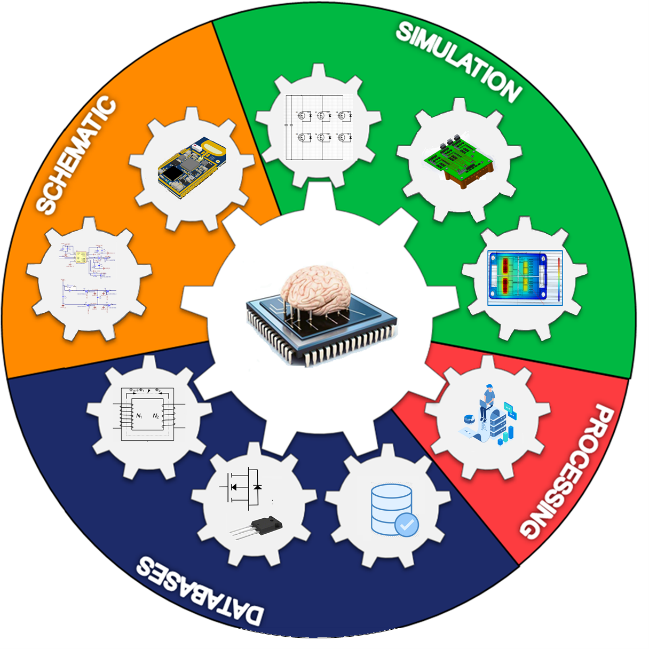
\includegraphics[width=6cm]{sample_figure.png} % Replace with your figure file
%     \caption{Sample figure.}
%     \label{fig:sample}
% \end{figure}

% \section{SECOND SECTION}
% Enter text, equations, and figures for your second full section here. Repeat as necessary for other sections. Equations should be expressed in the following format:

% \begin{equation}
%     A = \pi r^2
% \end{equation}

% \section{CONCLUSIONS AND FUTURE WORK}
% State your conclusions here and your plans for the final submission of a full paper, assuming your digest is accepted. Please clearly state your contributions compared with previous works, and list relevant references in the following \textbf{REFERENCES} section.

% You are reminded that the reviewers will prize experimental results and real-world applications, and as such, you should be sure to address these points in your digest. Evidence of completed experimental work will naturally be prized more than promises of future experimental work.

% \textbf{IMPORTANT:} This section is the last section in your five-page limit. If you let content bleed onto the sixth page, your submission will be automatically \textbf{REJECTED}.

% \newpage
% {\color{red}Note: references are required. This section should start on a separate page and it is not included in the five-page limit.  References can be single-spaced.References to articles can be made using \verb|\cite{b1,b2,b3}| e.g. \cite{b1,b2,b3}.}
% \bibliographystyle{IEEEtran}
% \bibliography{References}

% \vspace{30pt}
% {\color{red}Alternatively, the incorporation of input references may be executed as follows:}

% \begin{thebibliography}{00}

% \bibitem{b1} J. Doe, J.F. Stevens, and B. Smith, ``Title of their journal paper,'' \textit{Journal Title}, vol. 17, no. 1, pp. 123--133, Feb. 2005.
% \bibitem{b2} N. Surname and N. Surname, ``Title of their conference paper,'' in \textit{IEEE 1997 Conference Name}, 2017, pp. 122--129.
% \bibitem{b3} A.C. Doyle, \textit{Title of book}, Publisher’s Name, City, 2020.
% \end{thebibliography}
% \vspace{12pt}
% \end{document}
\documentclass[conference,onecolumn,a4paper,12pt,english,nofonttune]{IEEEtran}
\IEEEoverridecommandlockouts

% --- Packages for formatting ---
\usepackage[a4paper, margin=2.5cm]{geometry} % Sets 2.5 cm margins
\usepackage{setspace} % For double spacing
\usepackage{cite}
\usepackage{amsmath,amssymb,amsfonts}
\usepackage{algorithmic}
\usepackage{graphicx}
\usepackage{textcomp}
\usepackage{xcolor}
\def\BibTeX{{\rm B\kern-.05em{\sc i\kern-.025em b}\kern-.08em
    T\kern-.1667em\lower.7ex\hbox{E}\kern-.125emX}}

% --- Apply double spacing ---
\doublespacing
    
\begin{document}

\title{Trends and Technologies in Environmental Monitoring: A Review of Sensors, Communication, and AI-Enabled Systems*}

\thanks{This work was supported by the National Council for Scientific and Technological Development (CNPq).}

\vspace{30pt}
\author{\IEEEauthorblockN{\color{red} THIS IS A BLIND REVIEW. DO NOT INCLUDE AUTHOR INFORMATION!!!}}
\vspace{30pt}

\maketitle

\begin{abstract}
Wireless Sensor Networks (WSNs) are foundational for addressing modern environmental monitoring challenges driven by climate change. This review provides an integrated analysis of the trends and challenges, examining sensing technologies for water, soil, and air, alongside communication protocols and best practices. We consolidate advances across sensors, networking, and system-level challenges, including energy efficiency, security, and the integration of the Artificial Intelligence of Things (AIoT). By bridging these multidisciplinary domains, this work serves as a foundational guide for future research and the development of next-generation monitoring systems.
\end{abstract}

\begin{IEEEkeywords}
Environmental monitoring, Wireless Sensor Networks, Internet of Things (IoT), LoRaWAN, Artificial Intelligence of Things (AIoT).
\end{IEEEkeywords}

\section{INTRODUCTION}
The increasing urbanization and climate change have diverse impacts on different layers of society, threatening individuals in vulnerable situations during disasters such as floods, or affecting agricultural production due to climatic variations \cite{jonkman_2005_global}. These phenomena highlight the need for monitoring systems that can provide more data on environmental conditions and help us monitor, analyze, and predict such events \cite{hall_2014_understanding}.

When we talk about environmental monitoring, we refer to a wide range of applications and devices. Particularly in remote and hard-to-reach areas, this represents a significant technical challenge. The vastness of these territories, combined with adverse environmental conditions and the growing demand for real-time data, requires technological solutions that are robust, cost-effective, and scalable \cite{chen_2013_natural, yellampalli_2021_wireless }.

While many reviews focus on specific aspects such as soil sensors or water level measurement, few provide an integrated perspective combining sensing technologies, communication infrastructures, energy efficiency, artificial intelligence, and security. This review addresses that gap by consolidating advances across soil, water, and air monitoring domains to highlight overlooked technologies and guide future research toward scalable, intelligent, and resilient environmental monitoring solutions.

\section{REVIEW OF SENSING TECHNOLOGIES}
A wide array of sensing technologies is available for environmental monitoring, each with distinct advantages and use cases. For **water level monitoring**, conventional methods like limnigraphs face reliability issues in harsh conditions \cite{santana_2024_development}. Non-contact ultrasonic sensors have been proven as a viable, low-cost option for short-range measurements \cite{mohammadrezamasoudimoghaddam_2024_a}, while LiDAR offers superior accuracy and range, though its performance can be temperature-dependent \cite{paul_2020_a}. For large-scale monitoring, satellite-based remote sensing provides high consistency with in-situ data \cite{jiang_2024_monitoring, ali_2024_satellite}.

In **water quality**, recent developments include WSN nodes that use embedded machine learning to classify pollutants based on pH, turbidity, and EC sensor data \cite{ferreira_2023_conception}. For **soil monitoring**, batteryless technologies using NFC \cite{boada_2018_batteryless} and advanced optical fiber methods like AH-OFDR \cite{sun_2024_highresolution} are emerging. Finally, for **air quality and chemical detection**, Surface Acoustic Wave (SAW) sensors show promise for detecting gases and vapors \cite{devkota_2017_saw}, while reviews of low-cost sensors (LCS) confirm their potential to expand spatial coverage for monitoring pollutants like CO, O$_3$, and PM$_{2.5}$ \cite{karagulian_2019_review}.

\section{KEY CHALLENGES AND EMERGING TRENDS}
Beyond specific sensors, systemic challenges and trends shape the future of environmental monitoring. For **large area monitoring**, mobile data collection using vehicles equipped with RFID readers \cite{deng_2020_novel} or drones serving as LoRa gateways \cite{caruso_2021_drone} presents a scalable alternative to fixed WSNs.

In **power consumption**, "Beat sensors" represent an innovative, ultra-low-power paradigm where sensor data is encoded in the time interval between simple ID code transmissions. This approach has demonstrated a battery life of over seven years in some applications and has been adapted for solar-powered, battery-less water level monitoring with a 2 km LoRa range \cite{ishibashi_2017_beat, ishibashi_2019_long, dao_2025_lowcost}.

The integration of artificial intelligence, or **AIoT**, is a major trend, enabling smarter, context-aware sensors and predictive analytics \cite{ghosh_2018_artificial, mukhopadhyay_2021_artificial}. However, this integration elevates the importance of **security and privacy**. The constrained nature of embedded systems often leads to security being an afterthought, creating vulnerabilities to both software and hardware-level attacks that can compromise entire networks \cite{pimentel_2017_exploring, koulamas_2018_realtime, fournaris_2017_exploiting}.

\section{CONCLUSIONS AND CONTRIBUTIONS}
This review consolidates recent advances across a wide spectrum of environmental monitoring technologies, providing an integrated perspective that connects sensor development with communication infrastructures and systemic challenges. We identify a clear trend towards more autonomous, intelligent, and energy-efficient systems capable of operating in remote and harsh environments.

Our analysis concludes that while sensor maturity is improving, the primary challenges are now shifting towards scalable data acquisition, robust security architectures, and the effective application of AI to extract value from collected data. The convergence of innovations like batteryless sensors, mobile data collection, and AIoT enables more resilient systems to meet the demands of climate adaptation and resource management. This work contributes by offering a multidisciplinary guide for researchers and engineers, highlighting a path forward for developing the next generation of intelligent environmental monitoring solutions.

% --- References start on a new page and are not included in the page/word limit ---
\newpage
\begin{thebibliography}{00}

\bibitem{jonkman_2005_global} S. N. Jonkman, 
``Global Perspectives on Loss of Human Life Caused by Floods,'' 
Natural Hazards, vol. 34, pp. 151--175, Feb. 2005. doi: 10.1007/s11069-004-8891-3.

\bibitem{hall_2014_understanding} J. Hall \textit{et al.}, 
``Understanding Flood Regime Changes in Europe: A State-of-the-Art Assessment,'' 
Hydrology and Earth System Sciences, vol. 18, pp. 2735--2772, Jul. 2014. doi: 10.5194/hess-18-2735-2014.

\bibitem{chen_2013_natural} D. Chen, Z. Liu, L. Wang, M. Dou, J. Chen, and H. Li, 
``Natural Disaster Monitoring with Wireless Sensor Networks: A Case Study of Data-Intensive Applications upon Low-Cost Scalable Systems,'' 
Mobile Networks and Applications, vol. 18, pp. 651--663, Aug. 2013. doi: 10.1007/s11036-013-0456-9.

\bibitem{yellampalli_2021_wireless} S. Yellampalli, 
*Wireless Sensor Networks - Design, Deployment and Applications*, IntechOpen, Sep. 2021. doi: 10.5772/intechopen.77917. [Online]. Available: https://www.intechopen.com/books/8086

\bibitem{santana_2024_development} V. Santana, R. E. Salustiano, and R. Tiezzi, ``Development and Calibration of a Low-Cost LIDAR Sensor for Water Level Measurements,'' \emph{Flow Measurement and Instrumentation}, vol. 2024, pp. 102729--102729, Oct. 2024. doi: 10.1016/j.flowmeasinst.2024.102729.

\bibitem{mohammadrezamasoudimoghaddam_2024_a} M. MasoudiMoghaddam, J. Yazdi, and M. Shahsavandi, 
``A Low-Cost Ultrasonic Sensor for Online Monitoring of Water Levels in Rivers and Channels,'' 
Flow Measurement and Instrumentation, vol. 102, p. 102777, Dec. 2024. Elsevier BV. doi: 10.1016/j.flowmeasinst.2024.102777.

\bibitem{pereira_2022_evaluation} T. S. R. Pereira, T. P. de Carvalho, T. A. Mendes, and K. T. M. Formiga, 
``Evaluation of Water Level in Flowing Channels Using Ultrasonic Sensors,'' 
Sustainability, vol. 14, p. 5512, May 2022. doi: 10.3390/su14095512.

\bibitem{bresnahan_2023_a} P. Bresnahan, E. Briggs, B. Davis, A. Rodriguez, L. Edwards, C. Peach, N. Renner, H. Helling, and M. Merrifield, 
``A Low-Cost, DIY Ultrasonic Water Level Sensor for Education, Citizen Science, and Research,'' 
Oceanography, vol. 36, 2023. doi: 10.5670/oceanog.2023.101.

\bibitem{paul_2020_a} J. D. Paul, W. Buytaert, and N. Sah, 
``A Technical Evaluation of Lidar-Based Measurement of River Water Levels,'' 
Water Resources Research, vol. 56, Apr. 2020. doi: 10.1029/2019wr026810.

\bibitem{tamari_2016_flash} S. Tamari and V. Guerrero-Meza, 
``Flash Flood Monitoring with an Inclined Lidar Installed at a River Bank: Proof of Concept,'' 
Remote Sensing, vol. 8, p. 834, Oct. 2016. doi: 10.3390/rs8100834.

\bibitem{jiang_2024_monitoring} Z. Jiang and L. Hong, 
``Monitoring of Surface Water Area and Water Level Changes in Nine Plateau Lakes in Yunnan and Analysis of Influencing Factors,'' 
in *Proc. 2024 IEEE 6th Advanced Information Management, Communicates, Electronic and Automation Control Conf. (IMCEC)*, 
pp. 1027--1031, May 2024. doi: 10.1109/imcec59810.2024.10575197.

\bibitem{ali_2024_satellite} T. Ali, A. Zaidi, J. Rehman, F. Noor, F. Naz, and S. Jamali, 
``Satellite Radar Altimetry Insights into Dam-Induced Changes and Accuracy of Water Level Estimation for the Mekong River,'' 
in *Proc. IGARSS 2022 - IEEE Int. Geosci. Remote Sens. Symp.*, vol. 570, pp. 5063--5066, Jul. 2024. 
doi: 10.1109/igarss53475.2024.10642418.

\bibitem{ali_2020_saw} S. F. Ali, N. Mandal, P. Maurya, and A. Lata, 
``SAW Sensor Based a Novel Hydrostatic Liquid Level Measurement,'' 
in *Proc. IECON 2020 - 46th Annual Conf. IEEE Industrial Electronics Society*, pp. 724--729, Oct. 2020. 
doi: 10.1109/iecon43393.2020.9254540.

\bibitem{sreejith_2024_modeling} V. S. Sreejith and H. Zhang, 
``Modeling and Testing of a Highly Sensitive Surface Acoustic Wave Pressure Sensor for Liquid Depth Measurements,'' 
Sensors and Actuators A: Physical, vol. 372, p. 115377, Jul. 2024. doi: 10.1016/j.sna.2024.115377.

\bibitem{ramos_2025_high} C. C. Ramos, J. Preizal, X. Hu, C. Caucheteur, G. Woyessa, O. Bang, A. M. Rocha, and R. Oliveira, 
``High Resolution Liquid Level Sensor Based on Archimedes’ Law of Buoyancy Using Polymer Optical Fiber Bragg Gratings,'' 
Measurement, vol. 252, p. 117368, Mar. 2025. Elsevier BV. doi: 10.1016/j.measurement.2025.117368.

\bibitem{ferreira_2023_conception} Y. Ferreira, C. Silvério, and J. Viana, 
``Conception and Design of WSN Sensor Nodes Based on Machine Learning, Embedded Systems and IoT Approaches for Pollutant Detection in Aquatic Environments,'' 
IEEE Access, vol. 11, pp. 117040--117052, Jan. 2023. doi: 10.1109/access.2023.3325760.

\bibitem{nr_2025_ai} W. B. N.R, S. Palarimath, H. Gunasekaran, S. W. Haidar, S. G. S. Subitha, and J. Sarmila, 
``AI Modeling and Water Quality Sensing Technique Proffers Water Security: An Open Review,'' 
in *Proc. 2022 Int. Conf. Electronics and Renewable Systems (ICEARS)*, pp. 1028--1034, Feb. 2025. doi: 10.1109/icears64219.2025.10940077.

\bibitem{boada_2018_batteryless} M. Boada, A. Lazaro, R. Villarino, and D. Girbau, 
``Battery-Less Soil Moisture Measurement System Based on a NFC Device With Energy Harvesting Capability,'' 
IEEE Sensors Journal, vol. 18, pp. 5541--5549, Jul. 2018. 
doi: 10.1109/jsen.2018.2837388.

\bibitem{sun_2024_highresolution} C. Sun, C.-S. Tang, F. Vahedifard, Q. Cheng, A. Dong, T.-F. Gao, and B. Shi, "High-resolution monitoring of soil infiltration using distributed fiber optic," J. Hydrol., vol. 640, p. 131691, Jul. 2024, doi: 10.1016/j.jhydrol.2024.131691.

\bibitem{devkota_2017_saw} J. Devkota, P. Ohodnicki, and D. Greve, 
``SAW Sensors for Chemical Vapors and Gases,'' 
Sensors, vol. 17, p. 801, Apr. 2017. 
doi: 10.3390/s17040801.

\bibitem{karagulian_2019_review} F. Karagulian, M. Barbiere, A. Kotsev, L. Spinelle, M. Gerboles, F. Lagler, N. Redon, S. Crunaire, and A. Borowiak, 
``Review of the Performance of Low-Cost Sensors for Air Quality Monitoring,'' 
Atmosphere, vol. 10, p. 506, Aug. 2019. doi: 10.3390/atmos10090506.

\bibitem{yi_2015_a} W. Yi, K. Lo, T. Mak, K. Leung, Y. Leung, and M. Meng, ``A survey of wireless sensor network based air pollution monitoring systems,'' \emph{Sensors}, vol. 15, pp. 31392--31427, Dec. 2015. doi: 10.3390

\bibitem{deng_2020_novel} F. Deng, P. Zuo, K. Wen, and X. Wu, 
``Novel soil environment monitoring system based on RFID sensor and LoRa,'' 
Computers and Electronics in Agriculture, vol. 169, p. 105169, Feb. 2020. doi: 10.1016/j.compag.2019.105169.

\bibitem{caruso_2021_drone} A. Caruso, S. Chessa, S. Escolar, J. Barba, and J. C. Lopez, “Collection of Data with Drones in Precision Agriculture: Analytical Model and LoRa Case Study,” IEEE Internet of Things Journal, vol. 2021, pp. 1–1, 2021, doi: 10.1109/JIOT.2021.3075561.

\bibitem{ishibashi_2017_beat} 
K. Ishibashi, R. Takitoge, and S. Ishigaki, 
"Beat sensors IoT technology suitable for energy saving," 
in *Proc. 2017 7th Int. Conf. on Integrated Circuits, Design, and Verification (ICDV)*, pp. 52--55, Oct. 2017. doi: 10.1109/icdv.2017.8188637.

\bibitem{ishibashi_2019_long} 
K. Ishibashi, R. Takitoge, D. Manyvone, N. Ono, and S. Yamaguchi, 
"Long battery life IoT sensing by Beat Sensors," 
in *Proc. 2019 IEEE Int. Conf. on Industrial Cyber Physical Systems (ICPS)*, pp. 430--435, May 2019. doi: 10.1109/icphys.2019.8780159.

\bibitem{dao_2025_lowcost} 
M.-H. Dao, K. Ishibashi, T.-A. Nguyen, D.-H. Bui, H. Hirayma, T.-A. Tran, and X.-T. Tran, 
"Low-cost, high accuracy, and long communication range energy-harvesting Beat Sensor with LoRa and $\Omega$-antenna for water-level monitoring,"
*IEEE Sensors Journal*, vol. 25, pp. 1--1, Jan. 2025. doi: 10.1109/jsen.2025.3533014.

\bibitem{ghosh_2018_artificial} A. Ghosh, D. Chakraborty, and A. Law, 
'Artificial Intelligence in Internet of Things,' 
CAAI Transactions on Intelligence Technology, vol. 3, pp. 208--218, Dec. 2018. doi: 10.1049/trit.2018.1008. [Online]. Available: https://ietresearch.onlinelibrary.wiley.com/doi/10.1049/trit.2018.1008

\bibitem{mukhopadhyay_2021_artificial} S. C. Mukhopadhyay, S. K. S. Tyagi, N. K. Suryadevara, V. Piuri, F. Scotti, and S. Zeadally, 
``Artificial Intelligence-Based Sensors for Next Generation IoT Applications: A Review,'' 
IEEE Sensors Journal, vol. 21, pp. 1--1, 2021. doi: 10.1109/jsen.2021.3055618.

\bibitem{pimentel_2017_exploring}
Pimentel, A. D. (2017). Exploring exploration: A tutorial introduction to embedded systems design space exploration. \textit{IEEE Design \& Test}, 1, 77--90. doi:10.1109/MDAT.2016.2626445.

\bibitem{koulamas_2018_realtime}
Koulamas, C., \& Lazarescu, M. (2018). Real-time embedded systems: Present and future. Electronics, 9, 205. doi:10.3390/electronics7090205.

\bibitem{tien_2017_internet} J. M. Tien, 
``Internet of Things, Real-Time Decision Making, and Artificial Intelligence,'' 
Annals of Data Science, vol. 4, pp. 149--178, May 2017.

\bibitem{fournaris_2017_exploiting}
Fournaris, A., Pocero Fraile, L., \& Koufopavlou, O. (2017). Exploiting hardware vulnerabilities to attack embedded system devices: A survey of potent microarchitectural attacks. Electronics,3, 52. doi:10.3390/electronics6030052.


\end{thebibliography}

\end{document}